%% Geometry of circles %%
% Question 6
\hlquestion Find the points where the circle 
$x^{2} + y^{2} - 10x - 10y + 40 = 0$ 
and the line 
$y + 2x = 10$
intersect. 
Find the equation of the tangent to the circle at each of the points 
of intersection. Find the point of intersection of these two tangents.

\begin{solution}
	BE note: $(50 - r^{2} = 40) \rightarrow r^{2} = 10$
	\[
		(x-5)^{2} + (y-5)^{2} = 1
	\]
	\[
		\therefore
		\text{centre} \; 
		(5, 5)
		,\; \text{radius} = 
		\sqrt{10}
	\]
	\underline{Part 1: find points of intersection}
	\[ 
		y + 2x = 10
		\rightarrow
		y = -2x + 10
	\]
	\par
	Sub $(y = -2x + 10)$ into $x^{2} + y^{2} - 10x - 10y + 40 = 0$
	\[
		\rightarrow
		x^{2} + (-2x+10)^{2} - 10x - 10(-2x + 10) + 40 = 0
	\]
	\[
		x^{2} + 4x^{2} - 40x + 100 - 10x + 20 x - 100 + 40 = 0
	\]
	\[
		5x^{2} - 30x + 40 = 0
	\]
	\[
		x^{2} - 7x + 8 = 0
	\]
	\[
		(x-4)(x-2) = 0
	\]
	\[
		x = 4 
		\quad \& \quad
		x = 2
	\]
	Sub into: 
	\[
		y = -2x + 10	
	\]
	\begin{multicols}{2}
		Intersection 1: when $x=4$,
		\[
			y = -2(4) + 10
			\; 
			(= 2)
		\]
		\[
			\underline{
				(4, 2)
				}
		\]
		Intersection 2: when $x=2$,
		\[
			y = -2(2) + 10
			\; 
			(= 6)
		\]
		\[
			\underline{
				(2, 6)
			}
		\]		
	\end{multicols}
	\underline{Part 2: calculate tangent at each point}
	\par
	We have 
	$(5, 5) \leftrightarrow (4, 2)$ 
	and 
	$(5, 5) \leftrightarrow (2, 6)$
	\newline
	Using
	\[
		m_{1} = \frac{y_{1}-y_{2}}{x_{1}-x_{2}}
		\quad \& \quad
		y = mx + c
	\]
	\begin{multicols}{2}
		$(5, 5) \leftrightarrow (4, 2)$ 
		\[
			m_{1} = \frac{5-2}{5-4}
		\]
		\[
			m_{1} = 3
		\]
		\[
			\underline{
				\therefore
				m_{2} = -\frac{1}{3}
			}	
		\]
		$(5, 5) \leftrightarrow (2, 6)$ 
		\[
			m_{1} = \frac{5-6}{5-2}
		\]
		\[
			m_{1} = -\frac{1}{3}
		\]
		\[
			\underline{
				\therefore
				m_{2} = 3
			}	
		\]
	\end{multicols}
	\begin{multicols}{2}
		For point $(4, 2)$:
		\[
			\rightarrow
			(2) = -\frac{1}{3} (4) + c
		\]
		% \[
		% 	c = 2 + \frac{4}{3}
		% \]
		\[
			c = \frac{10}{3}
		\]
		\[
			y = -\frac{1}{3}x + \frac{10}{3}
		\]
		\begin{equation}
			\underline{
				\therefore
				3y = -x + 10
			}
			\label{eq:M8_circ_q06_tangent_at_point_x4_y2}
		\end{equation}
		% \columnbreak{}
		For point $(2, 6)$:
		\[
			\rightarrow
			(6) = 3 (2) + c
		\]
		\[
			c = 6 - 6
		\]
		\[
			c = 0
		\]
		\begin{equation}
			\underline{
				\therefore
				y = 3x
			}	
			\label{eq:M8_circ_q06_tangent_at_point_x2_y6}
		\end{equation}
	\end{multicols}
	\underline{Part 3: find intersection of two tangents}
	\newline
	Sub 
	\ref{eq:M8_circ_q06_tangent_at_point_x2_y6}
	into
	\ref{eq:M8_circ_q06_tangent_at_point_x4_y2}
	\[
		3(3x) = -x + 10
	\]
	\[
		10x = 10
	\]
	\[
		x = 1
		\quad \therefore \quad
		y = 3
	\]
	\qSolMath{
		(1, 3)
	}{}
	\underline{Diagram:}
	\begin{center}
		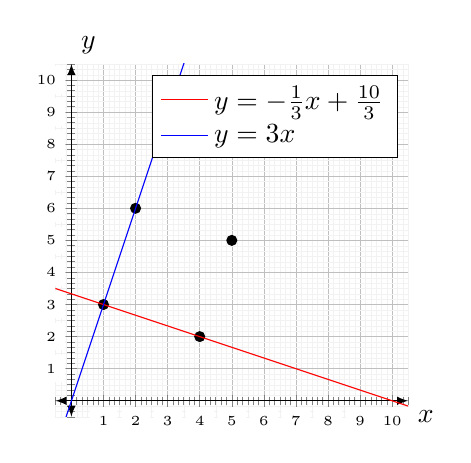
\begin{tikzpicture}
			\begin{axis}[
					width=0.5\textwidth,
					height=0.5\textwidth,
					xtick distance=1,
					ytick distance=1,
					xmin=0,xmax=10,
					ymin=0,ymax=10,
					xlabel = $x$,
					ylabel = $y$,
					grid=both,
					grid style={line width=.1pt, draw=gray!10},
					major grid style={line width=.2pt,draw=gray!50},
					axis lines=middle,
					minor tick num=5,
					enlargelimits={abs=0.5},
					axis line style={latex-latex},
					ticklabel style={font=\tiny,fill=white},
					xlabel style={at={(ticklabel* cs:1)},anchor=north west},
					ylabel style={at={(ticklabel* cs:1)},anchor=south west},
					legend pos=north east,
					legend entries={
						$y = -\frac{1}{3}x + \frac{10}{3}$,
						$y = 3x$,
					},
					legend cell align={left},
				]
				% circle
				\fill (axis cs: 5, 5) circle[radius=2pt];
				\draw (axis cs: 5, 5) circle[radius=31.622];%sqrt(10)=3.16227...
				% points
				\fill (axis cs: 4, 2) circle[radius=2pt];
				\fill (axis cs: 2, 6) circle[radius=2pt];

				\fill (axis cs: 1, 3) circle[radius=2pt];
				% lines
				\addplot[
					domain=-5:11, 
					samples=100, 
					color=red,
				]
				{ -(x/3) + (10/3) };
				\addplot[
					domain=-6:10, 
					samples=100, 
					color=blue,
				]
				{ (3*x) };
			\end{axis}
		\end{tikzpicture}
	\end{center}
		
\end{solution}

\appenddata{questionSolutions}{
{
	The points of intersection are $(4, 2)$ and $(2, 6)$. 
	The tangents are $3y + x = 10$ and $y = 3x$ respectively. 
	They intersect at the point $(1, 3)$
}
}